\documentclass{beamer}

\mode<presentation> {


\usetheme{default}
% \setbeamertemplate{footline} % To remove the footer line in all slides uncomment this line
\setbeamertemplate{footline}[page number] % To replace the footer line in all slides with a simple slide count uncomment this line
\setbeamertemplate{navigation symbols}{} % To remove the navigation symbols from the bottom of all slides uncomment this line
}

\usepackage{graphicx} % Allows including images
\usepackage{booktabs} % Allows the use of \toprule, \midrule and \bottomrule in tables
\usepackage{verbatim}
\usepackage{multicol}

\title[VE215 RC3]{VE215 RC4}
\author{Erdao Liang, Chongye Yang}
\institute[UM-SJTU JI] 
{UM-SJTU JI}
\date{\today}

\begin{document}

\AtBeginSection[ ]
{
\begin{frame}{Overview}
    \tableofcontents[sectionstyle=show/shaded,subsectionstyle=show/shaded/hide]
    % \tableofcontents[sectionstyle=show/shaded,subsectionstyle=show/shaded]
 \end{frame}
}

%%%%%%%%%%%%%%%%%%%%%%%%%%%%%%%%%%%%%%%%%%%%%%%%%%%
% TITLE PAGE
\begin{frame}
\titlepage % Print the title page as the first slide
\end{frame}

%%%%%%%%%%%%%%%%%%%%%%%%%%%%%%%%%%%%%%%%%%%%%%%%%%%
% OVERVIEW
% \begin{frame}
% \frametitle{Overview}
% \tableofcontents
% \end{frame}

\begin{frame}{From DC to AC}
    Begin our travel in alternating current circuits!
    \begin{itemize}
        \item Ch9: Introduce a new system to represent alternating signals
        \item Ch10: Analysis tools in AC context (with frequency $\omega$ fixed)
        \item Ch11: Analyze the how power is delivered in AC circuits
        \item Ch14: Investigate the circuit behavior when frequency $\omega$ is changed
    \end{itemize}
\end{frame}


%%%%%%%%%%%%%%%%%%%%%%%%%%%%%%%%%%%%%%%%%%%%%%%%%%%
% SINUSOIDS AND PHASORS
\section{Sinusoids and Phasors}

%%%%%%%%%%%%%%%%%%%%%%%%%
\begin{frame}{Sinosoid}

A sinusoid is a signal that has the form of sine or cosine function:
$$ v(t) = V_m \sin(\omega t + \phi)$$
where $V_m$ is the amplitude, $\omega$ is the frequency, and $\phi$ is the initial phase.

\vspace{1cm}

For $v_1(t)=V_m \sin(\omega t + \phi_1)$ and $v_2(t)=V_m\sin(\omega t + \phi_2)$,
\begin{itemize}
    \item If $\phi_1 = \phi_2$, $v_1$ and $v_2$ are \textbf{in phase}
    \item If $\phi_1 > \phi_2$, $v_1$ and $v_2$ are \textbf{out of phase}, $v_1$ \textbf{leads} $v_2$ and $v_2$ \textbf{lags} $v_1$
\end{itemize}

    
\end{frame}

%%%%%%%%%%%%%%%%%%%%%%%%%
\begin{frame}{Phasors}

Motivation: want a neat and simple way to represent sinusoidal signals, instead of $\cos$ and $\sin$.

Solution: use \textbf{phasor} to represent the $V_m$ (amplitude) and $\phi$ (phase) of a sinusoid.

\vspace{0.5cm}

Introducing complex number systems, we have
$$v(t) = V_m \sin(\omega t + \phi) = Re(V_me^{j(\omega t + \phi)}) = Re(\color{red}V_me^{j\phi}\color{black}e^{j\omega t})$$
Then we let
$${\color{red}\tilde{V} = V_me^{j\phi} = V_m \angle \phi}$$
This is the phasor representation of the sinusoid $v(t)$. Note that it doesn't keep the information of frequency $\omega$. We assume a fixed and known frequency from ch9 to ch13.

    
\end{frame}

%%%%%%%%%%%%%%%%%%%%%%%%%
\begin{frame}{Phasors}
Phasor representation:
\begin{itemize}
    \item \textbf{Polar form}: $\color{red}z = x + jy$
    \item \textbf{Rectangular form}: $\color{red}z = \vert z\vert \angle \theta$
    \item Conversion between each other::
    \begin{center}
    $R = \vert Z \vert \cos\theta, X = \vert Z \vert \sin \theta$
    
    $\vert Z \vert = \sqrt{R^2 + X^2}, \theta = \tan{(X/R)}$
    \end{center}
\end{itemize}

Phasor calculation:
\begin{itemize}
    \item Addition/subtraction more convenient in rectangular form:
    \begin{center}
        $z_1\pm z_2 = (x_1 \pm x_2) + j(y_1 \pm y_2)$
    \end{center}
    \item Multiplication/division more convenient in polar form:
    \begin{center}
        $z_1z_2 = \vert z_1 \vert \vert z_2\vert \angle (\phi_1 + \phi_2)$
        
        $\frac{z_1}{z_2} = \frac{\vert z_1 \vert}{ \vert z_2\vert}\angle (\phi_1 - \phi_2)$
        
    \end{center}
\end{itemize}
% Phasor diagram helps represent phasors graphically.

% \begin{figure}
%     \centering
%     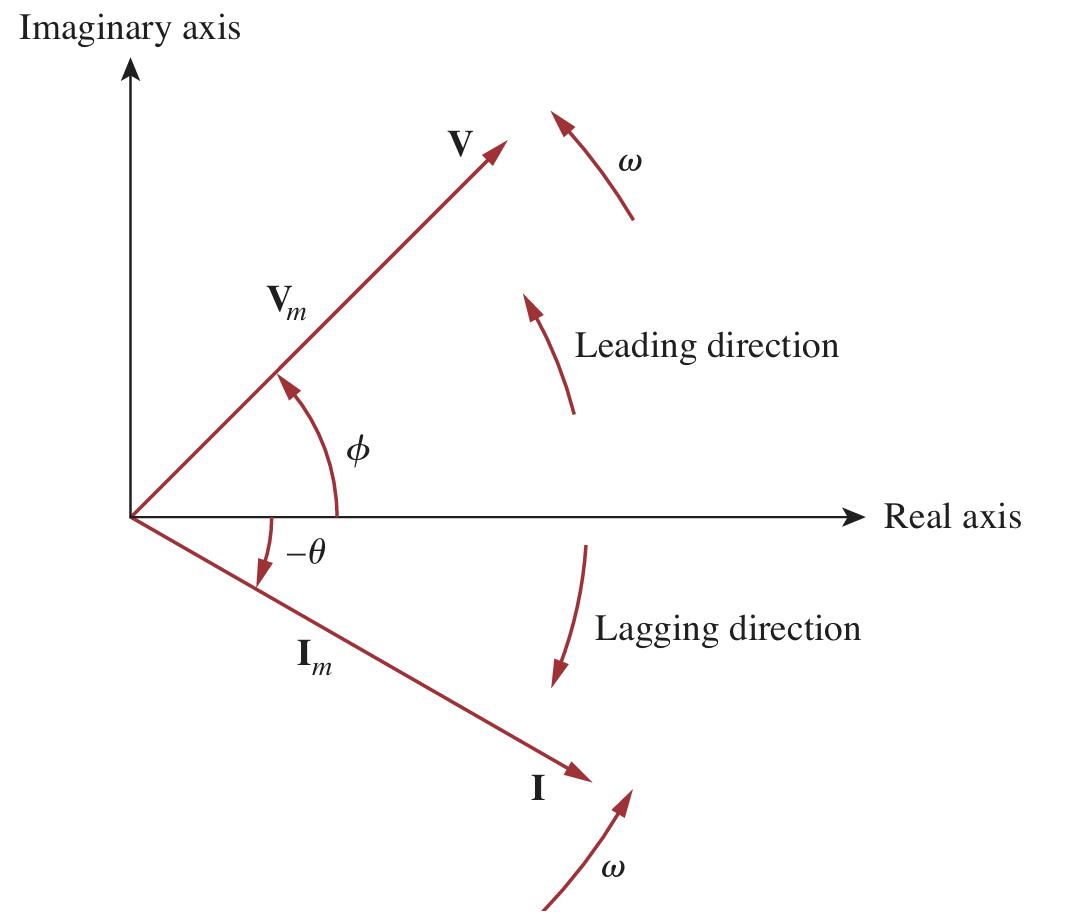
\includegraphics[width=0.5\textwidth]{img_ch9/1_phasor diagram.png}
% \end{figure}
    
\end{frame}

%%%%%%%%%%%%%%%%%%%%%%%%%
\begin{frame}{Phasor Relationships for Circuit Elements}

We can express the $I-V$ relationship of each type of circuit element in phasor context:

\begin{table}[]
    \centering
    \begin{tabular}{cccc}
        \toprule
        Element & Time domain & Phasor domain & Phase relationship\\
         \midrule
         Resistor & $v=Ri$& $\tilde{V} = R\tilde{I}$ & $I$, $V$ in phase\\
         Inductor & $v=L\frac{di}{dt}$ & \color{red} $\tilde{V} = j\omega L \tilde{I}$ & \color{red}$I$ lags $V$\\
         Capacitor & $i=C\frac{dv}{dt}$& \color{red}$\tilde{V} = \frac{1}{j \omega C}\tilde{I}$ & \color{red}$I$ leads $V$\\
         
         \bottomrule
    \end{tabular}
\end{table}

\begin{table}[]
    \centering
    \begin{tabular}{ccc}
         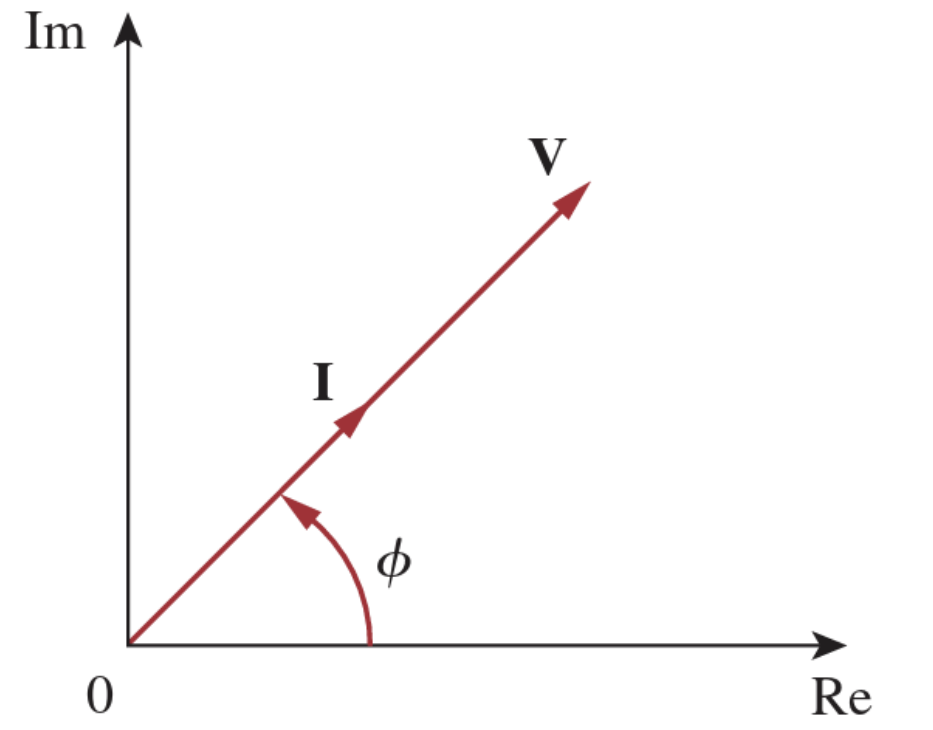
\includegraphics[width=0.27\textwidth]{img_ch9/5_phasordiagramR.png}
         & 
        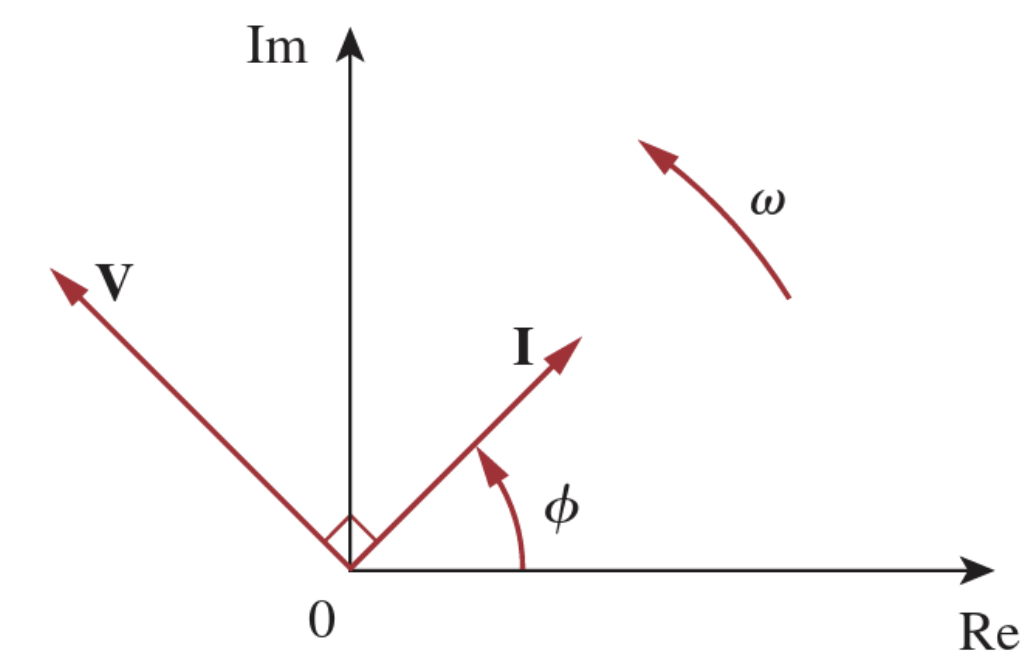
\includegraphics[width=0.32\textwidth]{img_ch9/6_phasordiagramL.png}
         &
        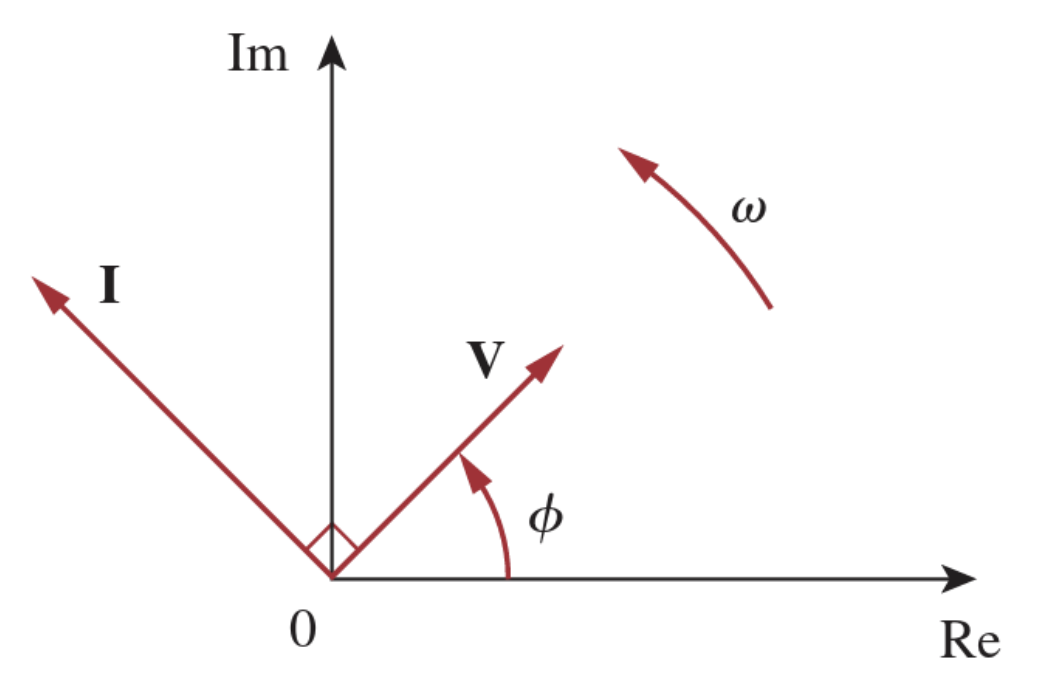
\includegraphics[width=0.32\textwidth]{img_ch9/7_phasordiagramC.png}
         \\
    \end{tabular}
\end{table}

\end{frame}

%%%%%%%%%%%%%%%%%%%%%%%%%
\begin{frame}{Impedance and Admittance}

\textbf{Impedance} $\color{red} Z = \tilde{V} / \tilde{I}$: a ``generalized" version of resistance.

$$Z = R\text{(resistance)} + jX\text{(reactance)} = \vert Z\vert\angle\theta$$
\begin{center}
    (unit in $\Omega$, same as resistance $R$)
\end{center}

\begin{table}[]
    \centering
    \begin{tabular}{cccc}
        \toprule
         Elements & Resistor & Inductor & Capacitor  \\
         \midrule
         Impedance $Z (\Omega)$ & $R$ & $j\omega L$ & $\frac{1}{j\omega C}$ \\
         Resistance $R (\Omega)$ & $R$ & 0 & 0 \\
         Reactance $X (\Omega)$ & 0 & $\omega L$ & $-\frac{1}{\omega C}$\\
         \bottomrule
    \end{tabular}
\end{table}
    
\end{frame}

%%%%%%%%%%%%%%%%%%%%%%%%%
\begin{frame}{Impedance and Admittance}

\textbf{Admittance} $Y = 1/Z$: a ``generalized" version of conductance.

$$Y = G\text{(conductance)} + jB\text{(susceptance)} = \vert Y\vert\angle\theta$$

\begin{center}
    (Unit in $S$, same as conductance $G$)
\end{center}

\begin{table}[]
    \centering
    \begin{tabular}{cccc}
        \toprule
         Elements & Resistor & Inductor & Capacitor  \\
         \midrule
         Impedance $Y (S)$ & $1/R$ & $-\frac{j}{\omega L}$ & $j\omega C$ \\
         Resistance $G (S)$ & $1/R$ & 0 & 0 \\
         Reactance $B (S)$ & 0 & $-\frac{1}{\omega L}$ & $\omega C$\\
         \bottomrule
    \end{tabular}
\end{table}


\end{frame}

%%%%%%%%%%%%%%%%%%%%%%%%%
\begin{frame}{Impedance Combination}

Previous rules still apply, only generalized.

\begin{table}[]
    \centering
    \begin{tabular}{ccc}
        \toprule
        & Series connection& Parallel connection \\
        \midrule
         Impedance $Z (\Omega)$ & $Z_{eq} = \sum_{i=1}^{n}Z_i$ & $\frac{1}{Y_{eq}} = \sum_{i=1}^{n}\frac{1}{Y_i}$\\
         Admittance $Y (S)$ & $\frac{1}{Z_{eq}} = \sum_{i=1}^{n}\frac{1}{Z_i}$ & $Y_{eq} = \sum_{i=1}^nY_i$ \\
         \bottomrule
    \end{tabular}
\end{table}

Capacitors and inductors are now treated similarly as resistors!
    
\end{frame}


%%%%%%%%%%%%%%%%%%%%%%%%%
\begin{frame}{Exercise}
Calculate $Z_{ab}$ in the figure below.

\begin{figure}
    \centering
    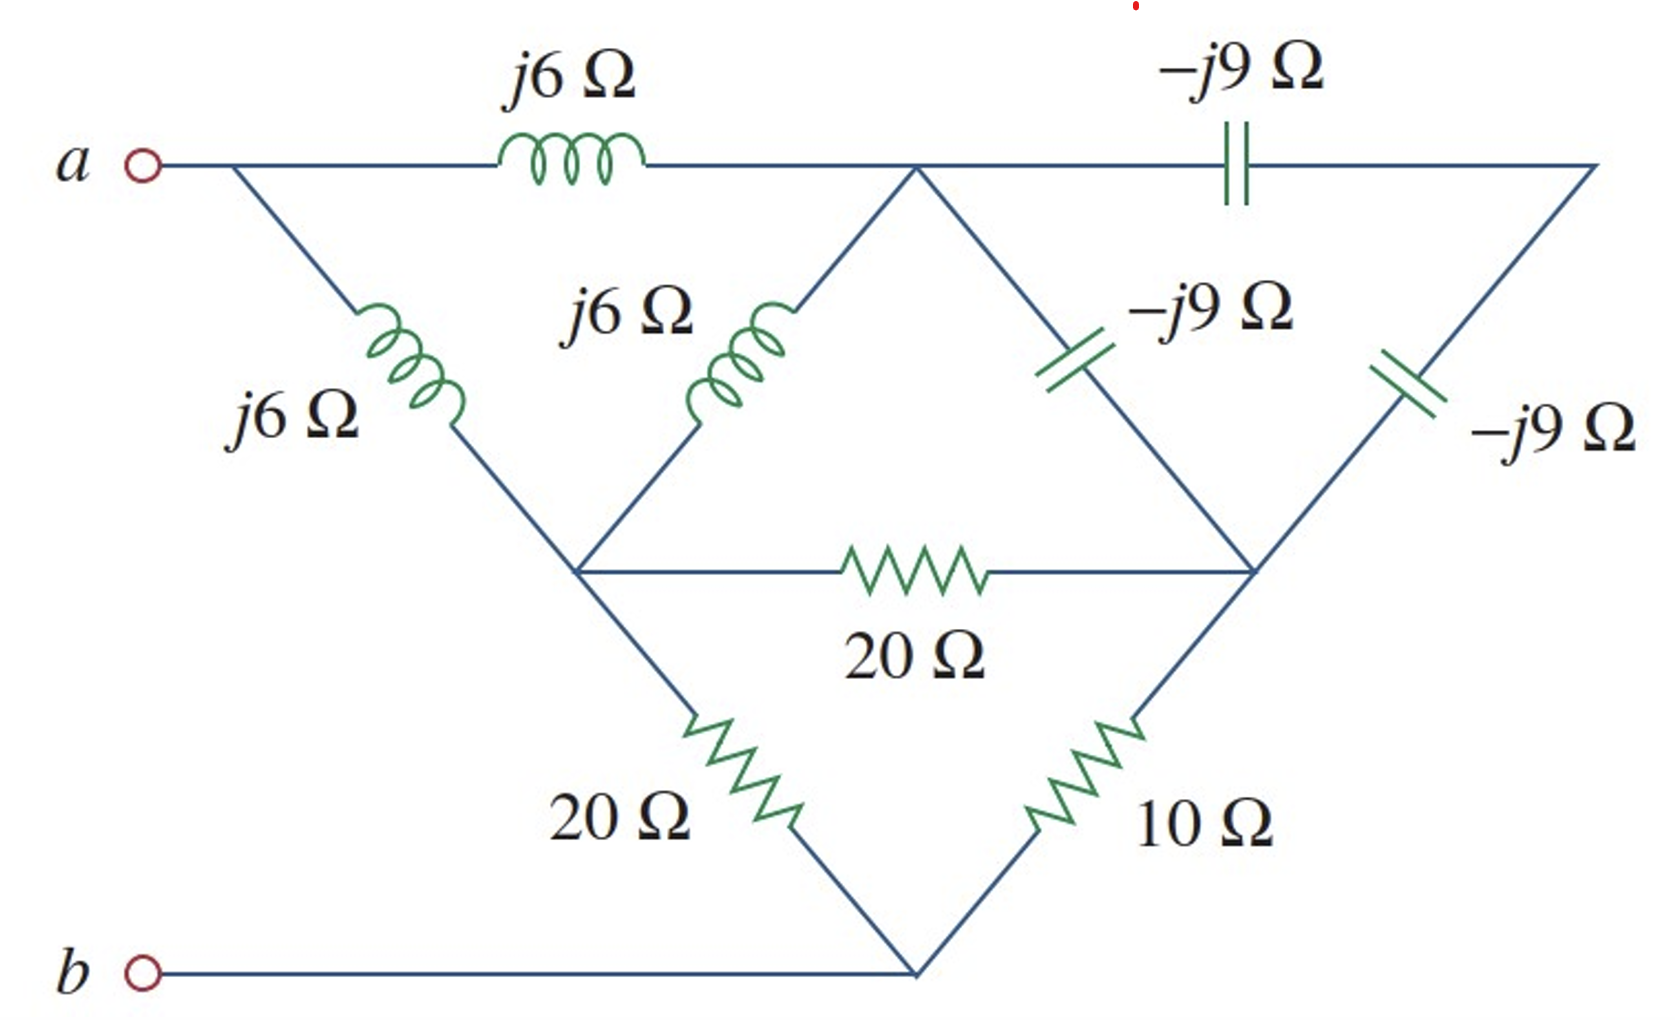
\includegraphics[width=0.65\textwidth]{img_ch9/exercise.png}
\end{figure}
    
\end{frame}

%%%%%%%%%%%%%%%%%%%%%%%%%
\begin{frame}{Exercise}
Calculate $Z_{ab}$ in the figure below.

\begin{figure}
    \centering
    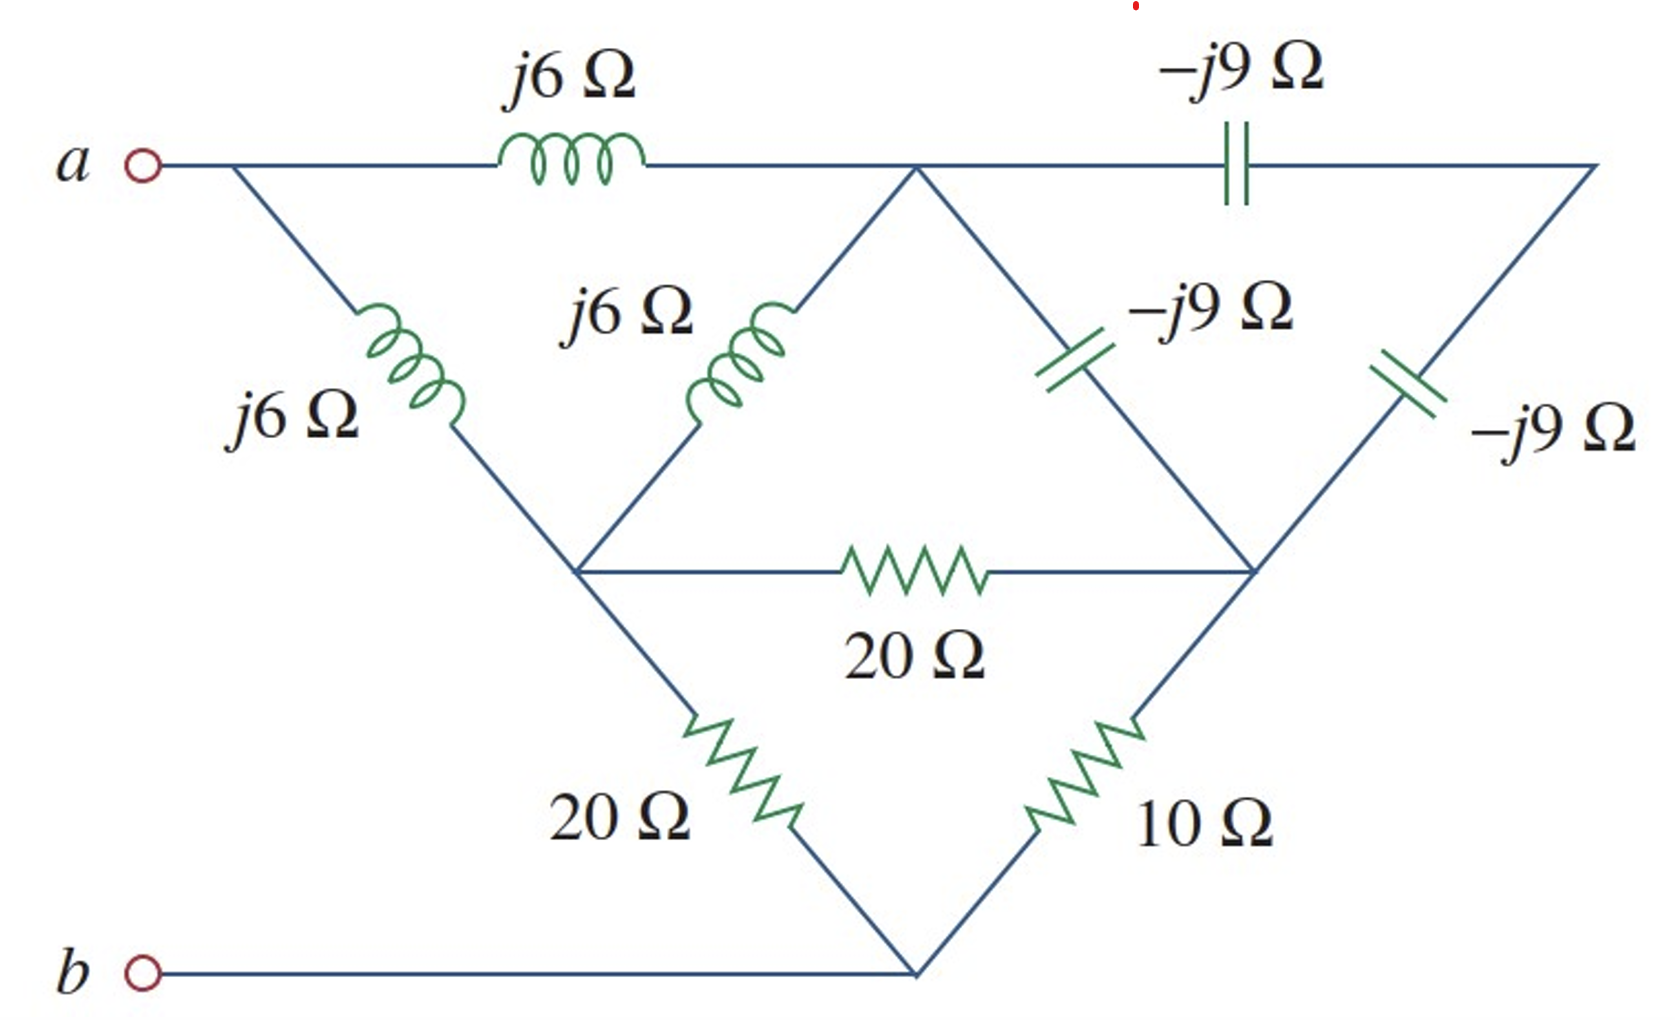
\includegraphics[width=0.65\textwidth]{img_ch9/exercise.png}
\end{figure}

Answer: $Z_{ab} = 7.57+j0.59=7.59\angle 4.49^{\circ} (\Omega)$
    
\end{frame}

%%%%%%%%%%%%%%%%%%%%%%%%%
\begin{frame}{Application: Phase Shifters}

Goal: change the phase of the original signal, lagging or leading

Solution: adopt an RC (or RL) circuit
\begin{table}[]
    \centering
    % \begin{s
    \begin{tabular}{cc}
        \toprule
        Leading shifter & Lagging shifter \\
        \midrule
        $V_o$ acorss resistor & $V_o$ across capacitor\\
        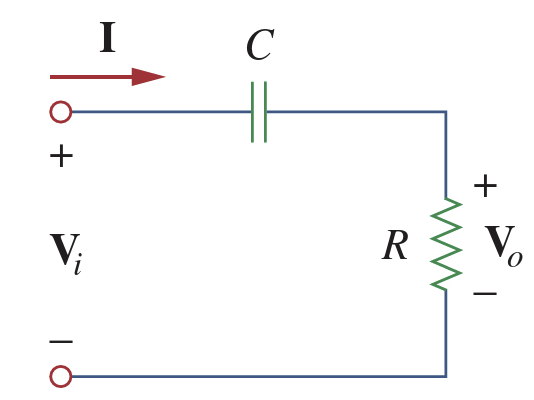
\includegraphics[width=0.32\textwidth]{img_ch9/3_shifterleadoutput.png}
        &
        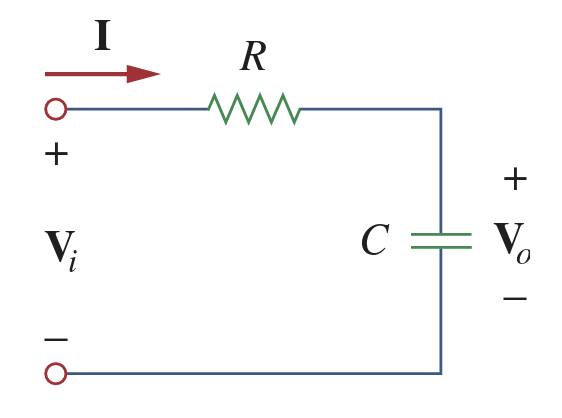
\includegraphics[width=0.33\textwidth]{img_ch9/4_shifterlagoutput.png}        
        \\
        \bottomrule
    \end{tabular}
\end{table}
    
\end{frame}

% Todo: 加公式
%%%%%%%%%%%%%%%%%%%%%%%%%
\begin{frame}{Application: Phase Shifters}
In a single shifter, $\color{red} 0 < \Delta\theta < 90^{\circ}$. Cascade shifters to achieve a $\geq 90^{\circ}$ phase shift.

\begin{figure}
    \centering
    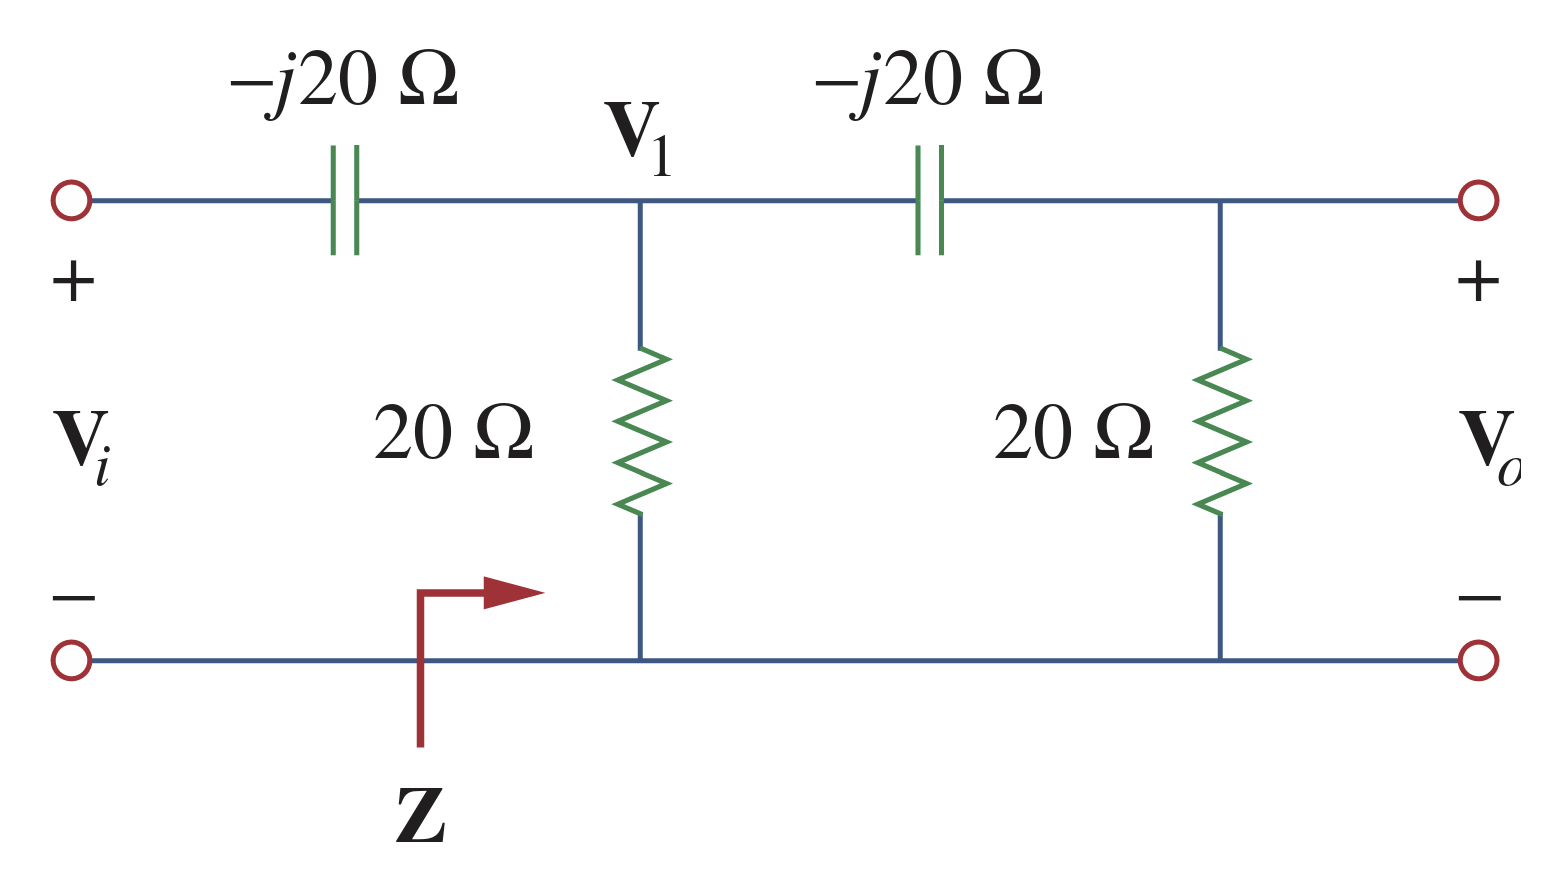
\includegraphics[width=0.6\textwidth]{img_ch9/8_cascadedshifter.png}
\end{figure}

$$TODO$$

\end{frame}

%%%%%%%%%%%%%%%%%%%%%%%%%%%%%%%%%%%%%%%%%%%%%%%%%%%
% SINUSOIDS STEADY-STATE ANALYSIS

\section{Sinusoidal Steady-State Analysis}

%%%%%%%%%%%%%%%%%%%%%%%%%
\begin{frame}{Sinusoidal Steady-State Analysis}

Basically, all the laws and methods we learned in DC circuit can still be applied in AC circuit.
\begin{itemize}
    \item Ohm’s Law
    \item KCL \& KVL
    \item Nodal \& Mesh Analysis
    \item $Y-\Delta$ Transformation
    \item \color{red}Superposition Theorem\color{black}
    \item Source Transformation
    \item Thevenin \& Norton Theorem
    \item Op-amp Circuits
\end{itemize}
    
\end{frame}

%%%%%%%%%%%%%%%%%%%%%%%%%
\begin{frame}{Importance of Superposition Theorem}

In a AC circuit, there might be sources operating at different frequencies. Analysis should be separate in each frequency, and added together with superposition theorem.

\begin{figure}
    \centering
    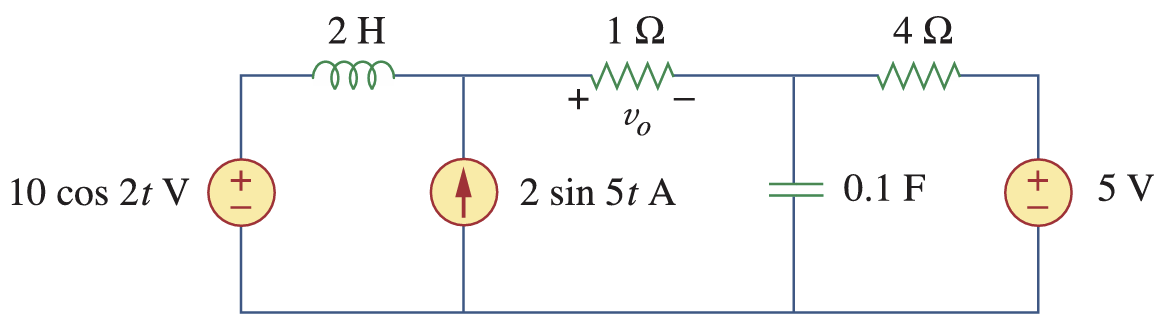
\includegraphics[width=0.7\textwidth]{img_ch10/1_example.png}
\end{figure}

\begin{figure}
    \centering
    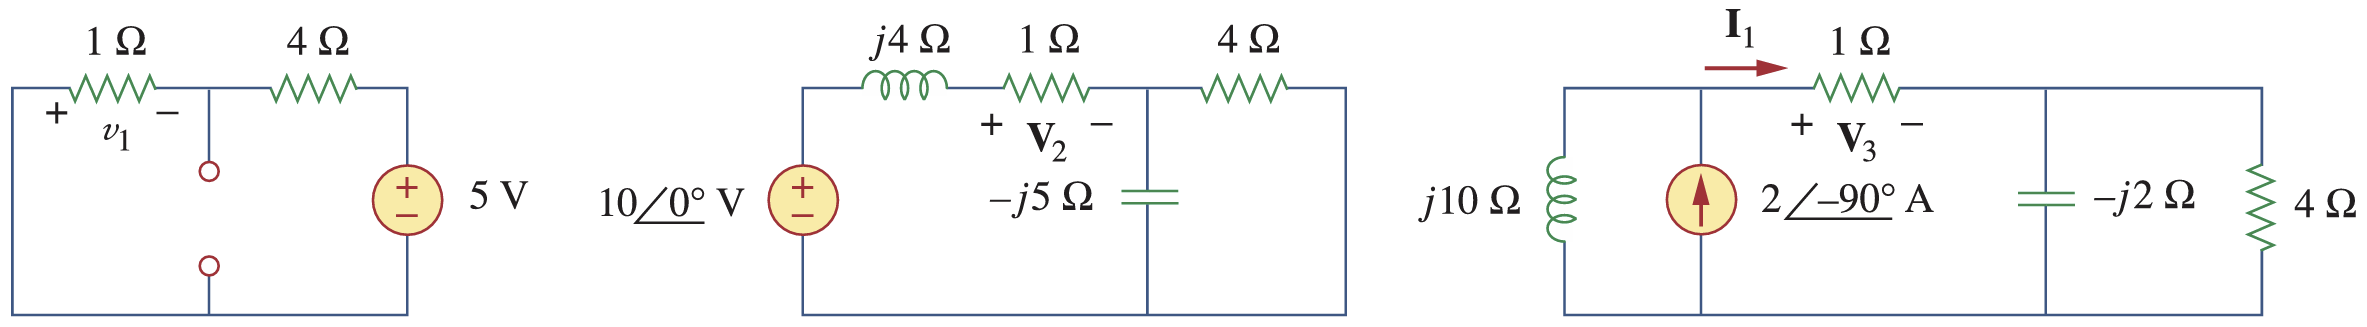
\includegraphics[width=\textwidth]{img_ch10/2_super.png}
\end{figure}
\begin{center}
    $v_o = v_1(\omega=0, \text{DC}) + v_2(\omega=2) + v_3(\omega=5) \quad\text{\color{red} in time domain}$
\end{center}

\end{frame}
 
%%%%%%%%%%%%%%%%%%%%%%%%%
\begin{frame}{Applications}

\begin{table}[]
    \centering
    \begin{tabular}{c|c}
        \textbf{Capacitance Multiplier}& \textbf{Oscillator} (Lab 7)  \\
        &\\
        Small capacitance + op-amp &  Produces an AC waveform as out-
          \\
         to produce large capacitance & put when powered by a DC input\\
         &\\
         ${I}_i/{V_i} = j\omega(1+\frac{R_2}{R_1})C$ &  ${Z}_p=R_2 \Vert \frac{1}{j\omega C_2} \quad Z_s = R_1 + \frac{1}{j\omega C_1}$\\

         ${Z}_i = {V}_i/{I}_i = \frac{1}{j\omega(1+R_2/R_1)C}$& $\text{gain} = \frac{V_2}{V_o} = \frac{Z_p}{Z_p+Z_s}=\frac{R_g}{R_f+R_g}$\\
        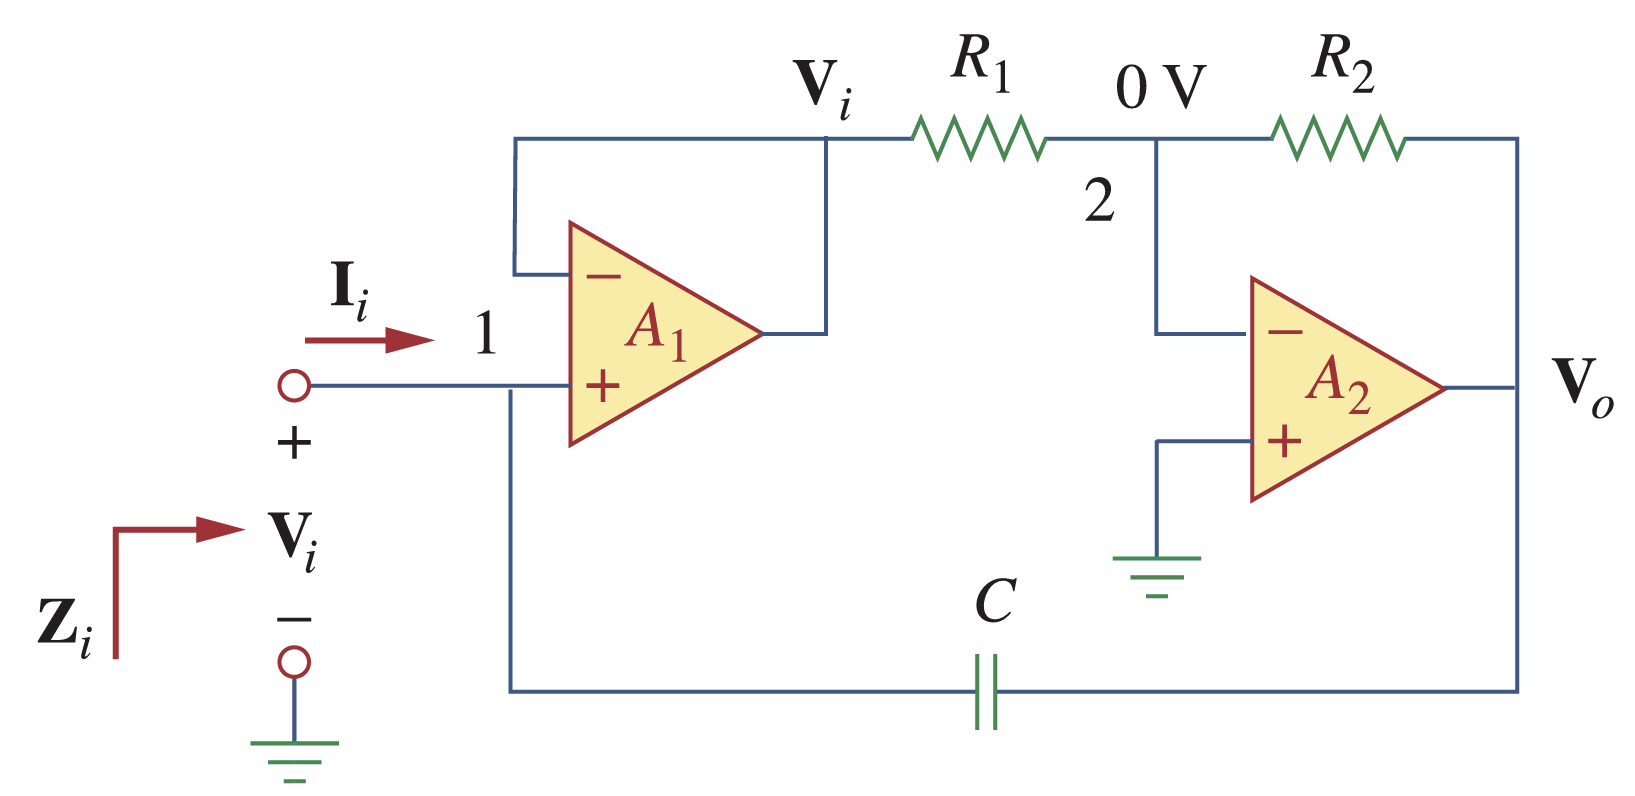
\includegraphics[width=0.4\textwidth]{img_ch10/3_capacitance multiplier.png}
         &
        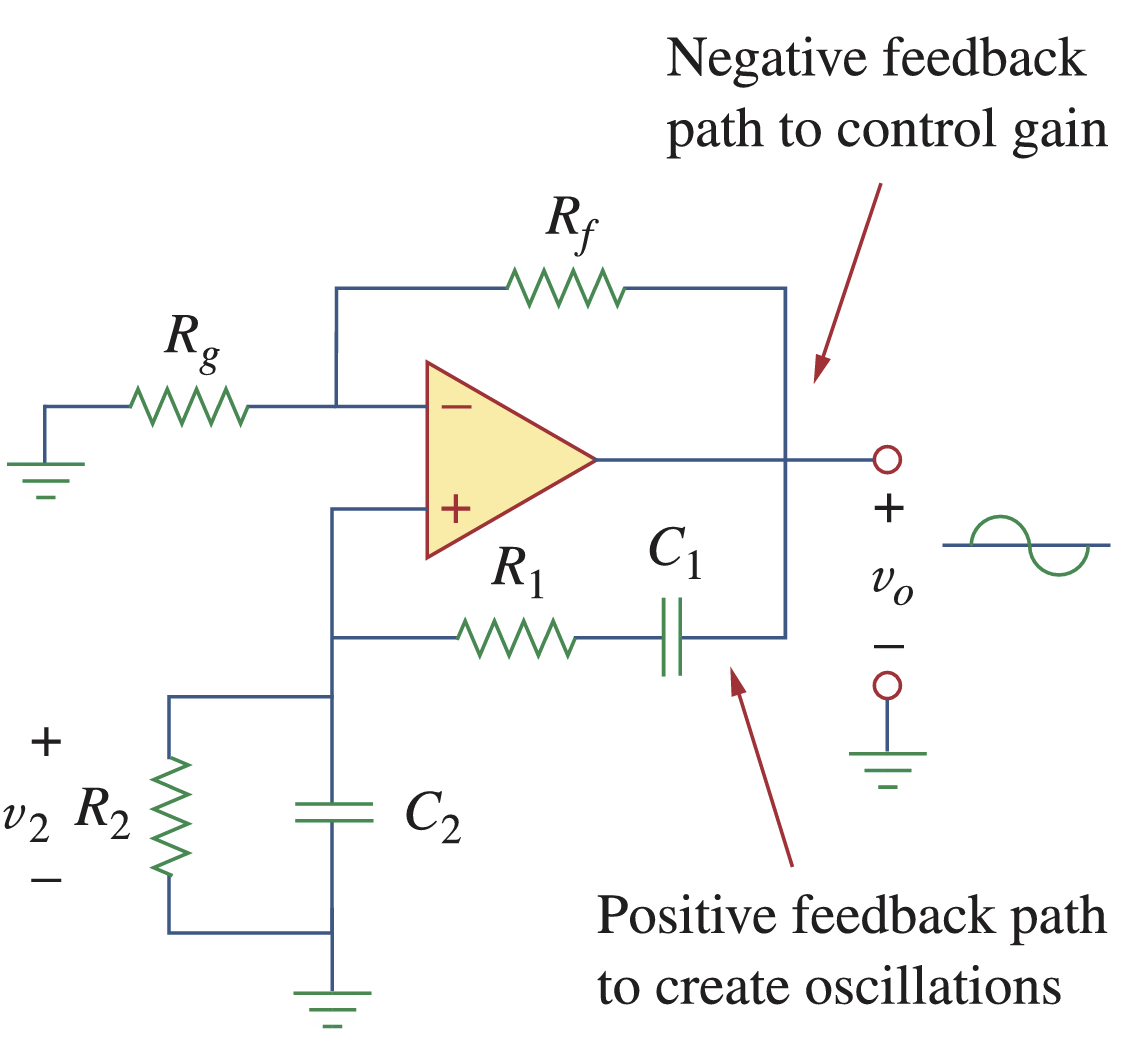
\includegraphics[width=0.35\textwidth]{img_ch10/4_oscillator.png}
         \\
    \end{tabular}
\end{table}

    
\end{frame}

%%%%%%%%%%%%%%%%%%%%%%%%%

\begin{frame}{Exercise}
    Find current $i(t)$ in the circuit below.
    \begin{figure}
        \centering
        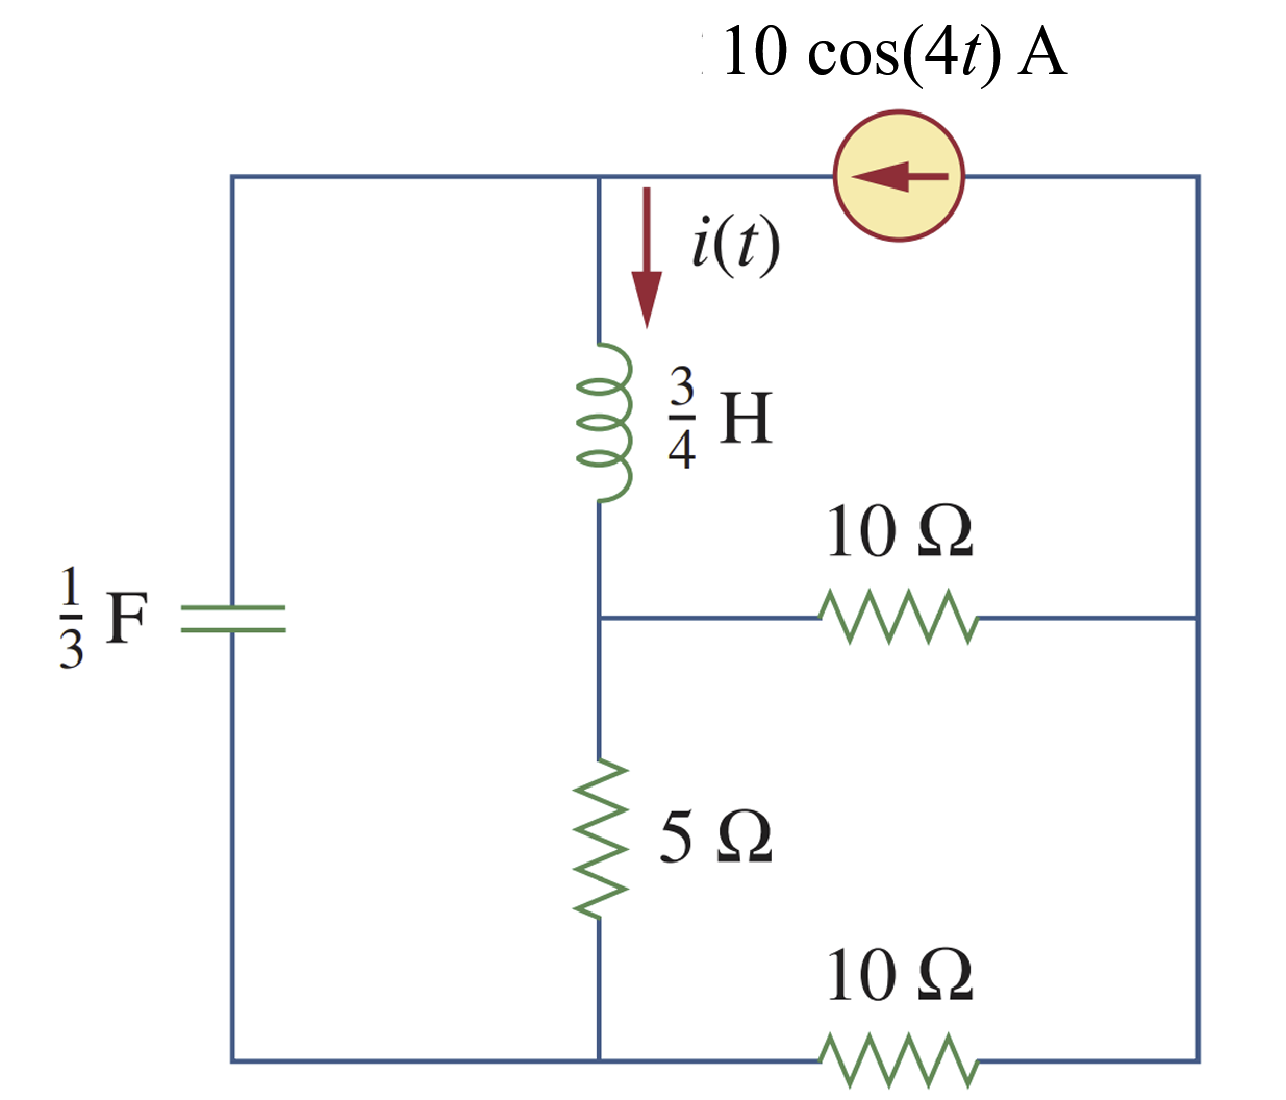
\includegraphics[width=0.55\textwidth]{img_ch10/exercise.png}
    \end{figure}
\end{frame}

%%%%%%%%%%%%%%%%%%%%%%%%%

\begin{frame}{Exercise}
    Find current $i(t)$ in the circuit below.
    \begin{figure}
        \centering
        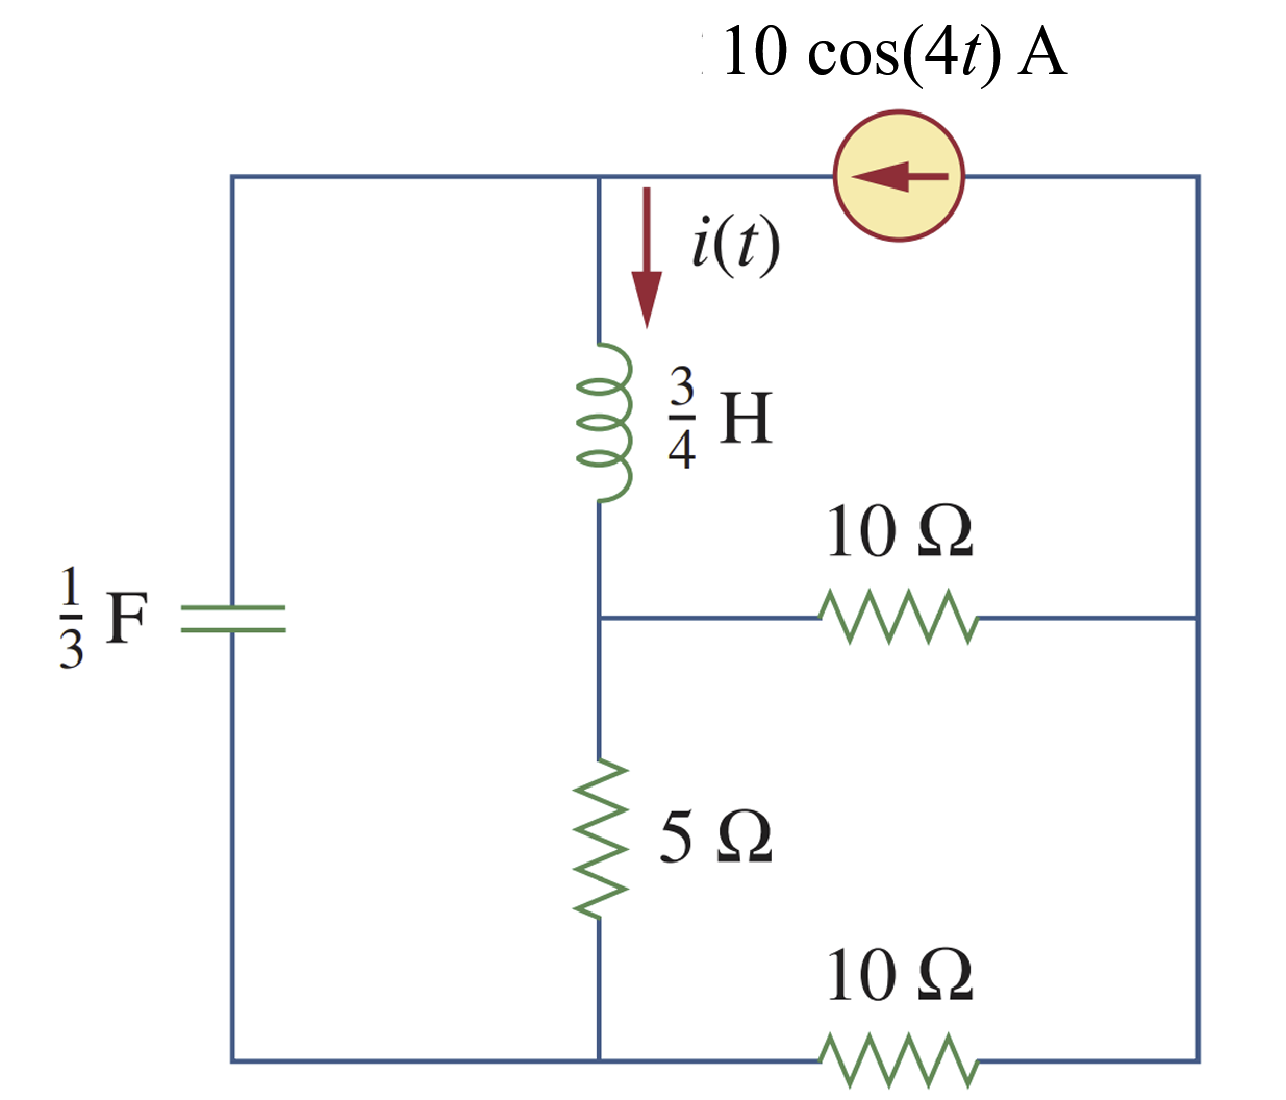
\includegraphics[width=0.55\textwidth]{img_ch10/exercise.png}
    \end{figure}
    
    Answer: $\mathbf{I} = 3.0-j3.56 \rightarrow i(t)=4.66\cos(4t-50.0^{\circ})$
\end{frame}


%%%%%%%%%%%%%%%%%%%%%%%%%%%%%%%%%%%%%%%%%%%%%%%%%%%
\begin{frame}
\frametitle{References}
\begin{enumerate}
\item 2023 Summer VE215 slides, Rui Yang
\item Fundamentals of Electric Circuits, 5th e, Sadiku, Matthew
\item 2022 Fall RC5, Yuxuan Peng
\item 2022 Fall RC6, Zhiyu Zhou
\end{enumerate}
\end{frame}


\begin{frame}
\Huge{\centerline{Thank you!}}
\end{frame}


\end{document}
